\chapter{Quantum speedup of the Travelling Salesman Problem for bounded-degree graphs}
\label{chp:tsp}

\section{Introduction}

Here we apply known quantum-algorithmic techniques to accelerate more recent classical TSP algorithms for the important special case of bounded-degree graphs. We say that a graph $G$ is degree-$k$ if the maximal degree of any vertex in $G$ is at most $k$. Although a sub-instance of the general Travelling Salesman Problem, this restriction is still NP-Hard for graphs of degree greater than 3 \cite{akiyama1980}.

A recent line of research has produced a sequence of algorithms which improve on the $O^*(2^n\log L)$ runtime of the general Held-Karp algorithm in this setting. First, Eppstein presented algorithms which solve the TSP on degree-3 graphs in time $O^*(2^{n/3}\log L) \approx O^*(1.260^n\log L)$, and on degree-4 graphs in time $O^*((27/4)^{n/3}\log L) \approx O^*(1.890^n\log L)$~\cite{eppstein2007}. The algorithms are based on the standard classical technique of {\em backtracking}, an approach where a tree of partial solutions is explored to find a complete solution to a problem (see Section \ref{sec:backtrack} for an introduction to this technique). Following subsequent improvements~\cite{iwama2007,liskiewicz14}, the best classical runtimes known for algorithms based on this general approach are $O^*(1.232^n\log L)$ for degree-3 graphs~\cite{xiao2016degree3}, and $O^*(1.692^n\log L)$ for degree-4 graphs~\cite{xiao2016degree4}, in each case due to Xiao and Nagamochi. All of these algorithms use polynomial space in $n$.

An algorithm of Bodlaender et al.~\cite{bodlaender15} achieves a faster runtime of $O^*(1.219^n\log L)$ for solving the TSP in degree-3 graphs, which is the best known; however, this algorithm uses exponential space. Similarly, an algorithm of Cygan et al.~\cite{cygan11} solves the TSP in unweighted degree-4 graphs in $O^*(1.588^n\log L)$ time and exponential space. Both of these algorithms use an approach known as cut-and-count, and a quantum speedup is not known for either algorithm.

In the case where we have an upper bound $L$ on the maximum edge cost in the graph, Bj\"orklund~\cite{bjorklund14} gave a randomised algorithm which solves the TSP on arbitrary graphs in $O^*(1.657^n L)$ time and polynomial space, which is an improvement on the runtime of the Xiao-Nagamochi algorithm for degree-4 graphs when $L$ is subexponential in $n$. Again, the techniques used in this algorithm do not seem obviously amenable to quantum speedup.

Here we use the quantum speedup to backtracking described in Section \ref{sec:q-backtrack} to speed up the algorithms of Xiao and Nagamochi in order to find Hamiltonian cycles shorter than a given upper bound, if such cycles do exist. We run this algorithm several times, using binary search to specify what our upper bound should be, in order to find the shortest Hamiltonian cycle and solve the Travelling Salesman Problem. In doing so, we achieve a near-quadratic reduction in the runtimes:

\begin{theorem}
There are bounded-error quantum algorithms which solve the TSP on degree-3 graphs in time $O^*(1.110^n \log^2 L \log \log L)$ and on degree-4 graphs in time $O^*(1.301^n \log^2 L \log \log L)$, where $L$ is the maximum edge cost. The algorithms use $\poly(n)\log L$ space.
\label{thm:deg34}
\end{theorem}

In this result and elsewhere in the chapter, ``bounded-error'' means that the probability that the algorithm either doesn't find a Hamiltonian cycle when one exists or returns a non-optimal Hamiltonian cycle is at most $1/3$. This failure probability can be reduced to $\delta$, for arbitrary $\delta > 0$, by repeating the algorithm $O(\log 1/\delta)$ times. Also here and throughout, $\log$ denotes $\log$ base 2. Note that the time complexity of our algorithms has some dependence on $L$, the largest edge cost in the input graph. However, this dependence is quite mild. For any graph whose edge costs are specified by $w$ bits, $L \le 2^w$. Thus terms of the form $\polylog(L)$ are at most polynomial in the input size.

Next, we show that degree-5 and degree-6 graphs can be dealt with via a randomised reduction to the degree-4 case.

\begin{theorem}
\label{thm:deg6}
There is a bounded-error quantum algorithm which solves the TSP on degree-5 and degree-6 graphs in time $O^*(1.680^n\log^2 L \log \log L)$. The algorithm uses $\poly(n)\log L$ space.
\end{theorem}

We summarise our results in Table \ref{tab:summary}.

\begin{table}
\begin{center}
\begin{tabularx}{\textwidth}{|c|c|C|c|}
\hline Degree & Quantum & Classical (poly space) & Classical (exp space) \\
\hline 3 & $O^*(1.110^n \polylog L)$ & $O^*(1.232^n\log L)$~\cite{xiao2016degree3} & $O^*(1.219^n\log L)$~\cite{bodlaender15} \\
 4 & $O^*(1.301^n \polylog L)$ & $O^*(1.692^n\log L)$~\cite{xiao2016degree4}, $O^*(1.657^n L)$~\cite{bjorklund14} & $O^*(1.588^n\log L)$~\cite{cygan11}\\
 5, 6 & $O^*(1.680^n \polylog L)$ & $O^*(1.657^n L)$~\cite{bjorklund14} & --- \\
\hline
\end{tabularx}
\end{center}
\caption[Runtimes of our quantum algorithms for the Travelling Salesman Problem]{Runtimes of our quantum algorithms for a graph of $n$ vertices with maximum edge cost $L$, compared with the best classical algorithms known.}
\label{tab:summary}
\end{table}

The rest of this chapter is as follows. In Section \ref{sec:tsp-related}, we introduce related work on quantum speedups for the Travelling Salesman problem when the graphs are of bounded degree. Then, in Section \ref{sec:bd}, we describe how this technique can be used to accelerate classical algorithms of Xiao and Nagamochi for graphs of degree at most 4~\cite{xiao2016degree3,xiao2016degree4}. In Section \ref{sec:higher-bound}, we extend this approach to graphs of degree at most 6.

\subsection{Related work}
\label{sec:tsp-related}

Surprisingly little work has been done on quantum algorithms for the TSP. D\"orn \cite{dorn2007} proposed a quantum speedup for the TSP for degree-3 graphs by applying amplitude amplification \cite{brassard1997} and quantum minimum finding~\cite{durr1996} to Eppstein's algorithm, and stated a quadratic reduction in the runtime. However, we were not able to reproduce this result (see Section~\ref{sec:backtrack-tsp} below for a discussion).

Very recently, Mandr{\`a}, Guerreschi and Aspuru-Guzik~\cite{mandra2016} developed a quantum algorithm for finding a Hamiltonian cycle in time $O(2^{(k-2)n/4})$ in a graph where {\em every} vertex has degree $k$. Their approach reduces the problem to an Occupation problem, which they solve via a backtracking process accelerated by the quantum backtracking algorithm~\cite{montanaro2015}. The bounds obtained from their algorithm are $O(1.189^n)$ for $k = 3$ and $O(1.414^n)$ for $k=4$, in each case a bit slower than the runtimes of our algorithms; for $k \ge 5$, their algorithm has a slower runtime than Bj\"orklund's classical algorithm~\cite{bjorklund14}.

% This degree of complexity suggests the problem as a candidate for quantum speedup, as even a modest improvement could result in a dramatic reduction in runtime. However, there has been little exploration of this problem from a quantum information perspective to date.


% ------------------------------------------------------------------------------

\section{Backtracking algorithms for the TSP}
\label{sec:backtrack-tsp}

The intuition behind why backtracking is a useful technique for solving the TSP is that we can attempt to build up a Hamiltonian cycle by determining for each edge in the graph whether it should be included in the cycle (``forced''), or deleted from the graph. As we add more edges to the cycle, we may either find a contradiction (e.g.\ produce a non-Hamiltonian cycle) or reduce the graph to a special case that can be handled efficiently (e.g.\ a collection of disjoint cycles of four unforced edges). This can sometimes allow us to prune the backtracking tree substantially.

To analyse the performance of backtracking algorithms for the TSP, a problem size measure is often defined that is at least 0 and at most $n$ (e.g.\ the number of vertices minus the number of forced edges). Note that if there are more than $n$ forced edges then it is impossible to form a Hamiltonian cycle that includes every forced edge, so the number of forced edges is at most $n$. At the start of the backtracking algorithm, there are no forced edges so the problem size is $n$. Each step of the backtracking algorithm reduces the problem size until the size is $0$, at which point either the $n$ forced edges form a Hamiltonian cycle or a Hamiltonian cycle that includes every forced edge cannot be found. A quasiconvex programming problem can be developed based on how the backtracking algorithm reduces the problem size. Solving this quasiconvex problem determines the number of recursive calls the backtracking algorithm needs to make before the problem size has been reduced to $0$. This is a runtime for the algorithm in terms of the problem size, which can be re-written in terms of $n$ due to the problem size being at most $n$.

It was proposed by D\"orn \cite{dorn2007} that amplitude amplification could be applied to speed up the runtime of Eppstein's algorithm for the TSP on degree-3 graphs~\cite{eppstein2007} from $O^*(2^{n/3}\log L)$ to $O^*(2^{n/6}\log L)$. Amplitude amplification can be used in this setting by associating a bit-string with each sequence of choices of whether to force or delete an edge, and searching over bit-strings to find the shortest valid Hamiltonian cycle. However, as suggested by the discussion in Section \ref{sec:q-backtrack}, a difficulty with this approach is that some branches of the recursion, as shown in Fig.~\ref{fig:size-decrease-by-two}, only reduce the problem size by 2 (as measured by the number of vertices $n$, minus the number of forced edges). The longest branch of the recursion can, as a result, be more than $n/3$ levels deep. In the worst case, this depth could be as large as $n/2$ levels. Specifying the input to the checking function $f$ could then require up to $n/2$ bits, giving a search space of size $O(2^{n/2})$. Under these conditions, searching for the solution via amplitude amplification could require up to $O^*(2^{n/4}\log L)$ time in the worst case. To yield a better runtime, we must take more of an advantage of the structure of our search space to avoid instances which will definitely not succeed.

The same issue with amplitude amplification applies to other classical algorithms for the TSP which are based on backtracking~\cite{xiao2016degree3,xiao2016degree4}. In the case of the Xiao-Nagamochi algorithm for degree-3 graphs, although the overall runtime bound proven for the problem means that the number of vertices in the tree is $O(2^{3n/10})$, several of the branching vectors used in their analysis have branches that reduce the problem size by less than $10/3$, leading to a branch in the tree that could be more than $3n/10$ levels deep.

\begin{figure}
\begin{center}
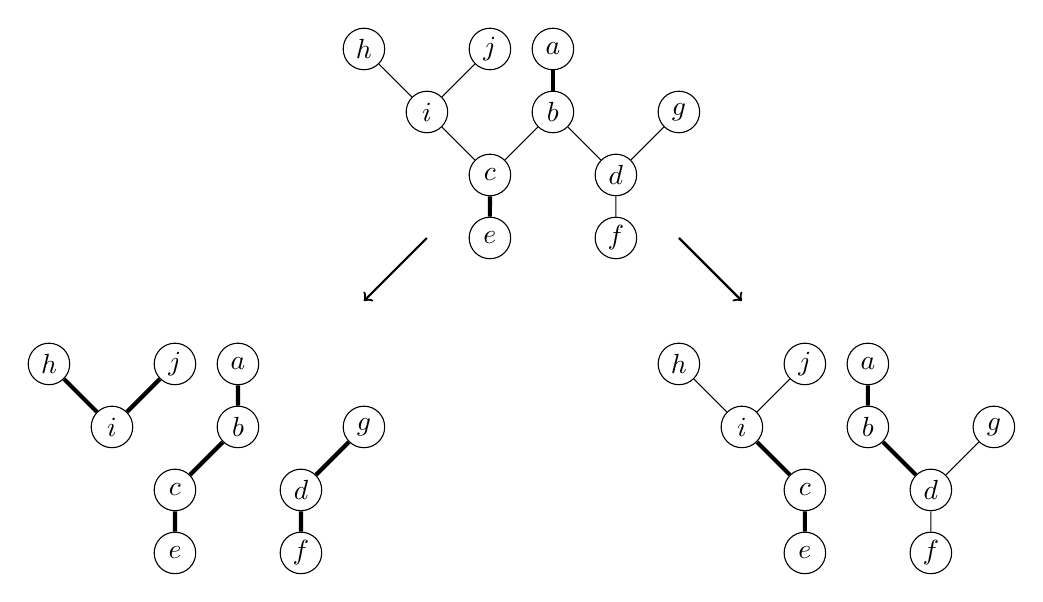
\begin{tikzpicture}[scale=0.8]
\tikzstyle{vertex}=[draw,shape=circle,inner sep=0pt,minimum size=15pt]
\path (0,0) node[vertex](f0){$a$};
\path (-2,-1) node[vertex](x0){$i$} (-1,-2) node[vertex](x1){$c$} (0,-1) node[vertex](f1){$b$} (1,-2) node[vertex](y1){$d$} (2,-1) node[vertex](y0){$g$};
\path (-1,-3) node[vertex](x2){$e$} (1,-3) node[vertex](y2){$f$};
\path (-3,0) node[vertex](x3){$h$} (-1,0) node[vertex](x4){$j$};
\draw[line width=1.5pt] (f0) -- (f1);
\draw[line width=1.5pt] (x2) -- (x1);
\draw (x0) -- (x1) -- (f1) -- (y1) -- (y2);
\draw (x3) -- (x0) -- (x4);
\draw (y0) -- (y1);

\path (-5,-5) node[vertex](f0){$a$};
\path (-7,-6) node[vertex](x0){$i$} (-6,-7) node[vertex](x1){$c$} (-5,-6) node[vertex](f1){$b$} (-4,-7) node[vertex](y1){$d$} (-3,-6) node[vertex](y0){$g$};
\path (-6,-8) node[vertex](x2){$e$} (-4,-8) node[vertex](y2){$f$};
\path (-8,-5) node[vertex](x3){$h$} (-6,-5) node[vertex](x4){$j$};
\draw[line width=1.5pt] (f0) -- (f1) -- (x1) -- (x2);
\draw[line width=1.5pt] (x3) -- (x0) -- (x4);
\draw[line width=1.5pt] (y2) -- (y1) -- (y0);

\path (5,-5) node[vertex](f0){$a$};
\path (3,-6) node[vertex](x0){$i$} (4,-7) node[vertex](x1){$c$} (5,-6) node[vertex](f1){$b$} (6,-7) node[vertex](y1){$d$} (7,-6) node[vertex](y0){$g$};
\path (4,-8) node[vertex](x2){$e$} (6,-8) node[vertex](y2){$f$};
\path (2,-5) node[vertex](x3){$h$} (4,-5) node[vertex](x4){$j$};
\draw[line width=1.5pt] (f0) -- (f1) -- (y1);
\draw[line width=1.5pt] (x0) -- (x1) -- (x2);
\draw (x3) -- (x0) -- (x4);
\draw (y0) -- (y1) -- (y2);

\draw[thick, ->] (-2,-3) -- (-3,-4);
\draw[thick, ->] (2,-3) -- (3,-4);
\end{tikzpicture}
\end{center}
\caption[An instance of the recursive step in Eppstein's algorithm]{An instance of the recursive step in Eppstein's backtracking algorithm for the TSP~\cite{eppstein2007} for a subgraph of a larger graph $G$, with forced edges displayed in bold and  branching on edge $bc$. If we force $bc$, then $b$ and $c$ are both incident to two forced edges, so $bd$ and $ci$ cannot be part of the Hamiltonian cycle and can be removed from the graph. After these edges are removed, vertices $i$ and $d$ are both of degree $2$, so in order to reach those vertices the edges $hi$, $ij$, $df$ and $dg$ must also be included in the Hamiltonian cycle. So forcing $bc$ has overall added five edges to the Hamiltonian cycle. On the other hand, if we remove edge $bc$, we find that $b$ and $c$ are vertices of degree $2$, so edges $bd$ and $ci$ must be part of the Hamiltonian cycle. Thus we have only added two more edges to the Hamiltonian cycle.
\label{fig:size-decrease-by-two}}
\end{figure}

% ------------------------------------------------------------------------------

\section{Quantum speedups for the Travelling Salesman Problem on bounded-degree graphs \label{sec:bd}}
\label{sec:deg3}

Our algorithms are based on applying the quantum algorithm for backtracking (Theorem \ref{thm:backtrack}) to Xiao and Nagamochi's algorithm for solving the TSP for degree-3 graphs~\cite{xiao2016degree3}. Before describing our algorithms, we need to introduce some terminology from~\cite{xiao2016degree3} and describe their original algorithm. The algorithm, and its analysis, are somewhat involved, so we omit details wherever possible.

\subsection{The algorithm of Xiao and Nagamochi}
\label{sec:xndeg3}

A graph $G$ is $k$-edge connected if there are $k$ edge-disjoint paths between every pair of vertices. An edge in $G$ is said to be forced if it must be included in the final tour, and unforced otherwise. The set of forced edges is denoted $F$, and the set of unforced edges is denoted $U$. An induced subgraph of unforced edges which is maximal and connected is called a $U$-component. If a $U$-component is just a single vertex, then that $U$-component is trivial. A maximal sequence $\mathcal{C}$ of edges in a $U$-component $H$ is called a circuit if either:
%
\begin{itemize}
\item $\mathcal{C} = \{xy\}$ and there are three edge-disjoint paths from $x$ to $y$,
\item or $\mathcal{C} = \{c_0, c_1,\dots,c_{m-1}\}$ such that for $0 \leq i < m-1$, there is a subgraph $B_i$ of $H$ such that the only two unforced edges incident to $B_i$ are $c_i$ and $c_{i+1}$.
\end{itemize}
%

A circuit is reducible if subgraph $B_i$ for some $i$ is incident to only two edges. In order for $B_i$ to be reached, both edges incident to $B_i$ need to be forced. Forcing one edge in the circuit then means that the other edges can be either forced or removed. The polynomial time and space process by Xiao and Nagamochi to reduce circuits, by forcing and removing alternating edges in the circuit, is known as the {\em circuit procedure} \cite{xiao2016degree3}.

Note that each edge can be in at most one circuit. If two distinct circuits $\mathcal{C}, \mathcal{C}'$ shared an edge $e_i$, then there are two possibilities. The first is that there is a subgraph $B_i$ incident to unforced edges $e_i \in \mathcal{C} \cap \mathcal{C}', e_{i+1} \in \mathcal{C} - \mathcal{C}', e_j \in \mathcal{C}' - \mathcal{C}$. In this case, $B_i$ is incident to more than two unforced edges, so neither $\mathcal{C}$ nor $\mathcal{C}'$ are circuits, which is a contradiction.

The second is that there is some edge $e_i$ which is incident to distinct subgraphs $B_i, B_i'$ related to $\mathcal{C}, \mathcal{C}'$, respectively. Circuits are maximal sequences, so it cannot be the case that $B_i$ is a subgraph of $B_i'$, otherwise $\mathcal{C}' \subseteq \mathcal{C}$. Now we consider the subgraphs $B_i \cap B_i'$ and $B_i - B_i'$, which must be connected by unforced edges as they are both subgraphs of $B_i$. These unforced edges are incident to $B_i'$, which is a contradiction as they are not part of $\mathcal{C}'$.

Let $X$ be a subgraph. We define $\text{cut}(X)$ to be the set of edges that connect $X$ to the rest of the graph. If $|\text{cut}(X)| = 3$, then we say that $X$ is $3$-cut reducible. It was shown by Xiao and Nagamochi~\cite{xiao2016degree3} that, if $X$ is 3-cut reducible, $X$ can be replaced with a single vertex of degree $3$ with outgoing edges weighted such that the length of the shortest Hamiltonian cycle is preserved.

The definition of $4$-cut reducible is more complex. Let $X$ be a subgraph such that $\text{cut}(X) \subseteq F$ and $|\text{cut}(X)| = 4$. A solution to the TSP would have to partition $X$ into two disjoint paths such that every vertex in $X$ is in one of the two paths. If $x_1, x_2, x_3$ and $x_4$ are the four vertices in $X$ incident to the four edges in $\text{cut}(X)$, then there are three ways these paths could start and end:
%
\begin{itemize}
\item $x_1 \leftrightarrow x_2$ and $x_3 \leftrightarrow x_4$,
\item $x_1 \leftrightarrow x_3$ and $x_2 \leftrightarrow x_4$,
\item or $x_1 \leftrightarrow x_4$ and $x_2 \leftrightarrow x_3$.
\end{itemize}
%
We say that $X$ is $4$-cut reducible if for at least one of the above cases it is impossible to create two disjoint paths in $X$ that include all vertices in $X$. Xiao and Nagamochi defined a polynomial time and space process for applying the above reductions, known as {\em $3/4$-cut reduction}~\cite{xiao2016degree3}.

A set of edges $\{e_i\}$ are {\em parallel} if they are incident to the same vertices (note that here we implicitly let $G$ be a multigraph; these may be produced in intermediate steps of the algorithm). If there are only two vertices in the graph, then the TSP can be solved directly by forcing the shortest two edges. Otherwise if at least one of the edges is not forced, then we can reduce the problem by removing the longer unforced edges until the vertices are only adjacent via one edge. This is the process Xiao and Nagamochi refer to as {\em eliminating parallel edges} \cite{xiao2016degree3}.

Finally, a graph is said to satisfy the parity condition if every $U$-component is incident to an even number of forced edges and for every circuit $\mathcal{C}$, an even number of the corresponding subgraphs $B_i$ satisfy that $|\text{cut}(B_i) \cap F|$ is odd.

%We will now explain how to speed up Xiao and Nagamochi's algorithm for graphs of bounded degree $3$. We shall start by proving the following lemma:

%\begin{lemma}
%Let $G$ be a graph of bounded degree $3$. There is a quantum algorithm which finds a Hamiltonian cycle in $G$ with probability $\delta$ in $O(2^{3n/20}\poly(n)\log(1/\delta))$.
%\label{thm:hamiltonian-cycle}
%\end{lemma}

%It is worth noting that Lemma \ref{thm:hamiltonian-cycle} beats the algorithm by Mandr{\`a}, Guerreschi and Aspuru-Guzik for finding a Hamiltonian cycle \cite{mandra2016}, which for bounded degree $3$ graphs runs in time $O(2^{n/4})$.

We are now ready to describe Xiao and Nagamochi's algorithm. The algorithm takes as input a graph $G = (V, E)$ and a set of forced edges $F \subseteq E$ and returns the length of the shortest Hamiltonian cycle in $G$ containing all the edges in $F$, if one exists.

The algorithm is based on four subroutines: {\em eliminating parallel edges}, the {\em 3/4-cut reduction}, {\em selecting a good circuit} and the {\em circuit procedure}, as well as the following lemma:

\begin{lemma}[Eppstein~\cite{eppstein2007}]
\label{lem:trivial}
If every $U$-component in a graph $G$ is trivial or a component of a 4-cycle, then a minimum cost tour can be found in polynomial time.
\end{lemma}

We will not define the subroutines here in any detail; for our purposes, it is sufficient to assume that they all run in polynomial time and space. The circuit procedure for a circuit $\mathcal{C}$ begins by either adding an edge $e \in \mathcal{C}$ to $F$ or deleting it from the graph, then performing some other operations. ``Branching on a circuit $\mathcal{C}$ at edge $e \in \mathcal{C}$'' means generating two new instances from the current instance by applying each of these two variants of the circuit procedure starting with $e$.

The Xiao-Nagamochi algorithm is described in Algorithm \ref{alg:tsp3}, reproduced from~\cite{xiao2016degree3}. Lines 2 and 3 check that the existence of a Hamiltonian cycle is not ruled out, by ensuring that that there are at least two disjoint paths between any pair of vertices and that the graph satisfies the parity condition. Lines 4 and 5 reduce any reducible circuit by initially forcing one edge and then alternately removing and forcing edges. Lines 6 \& 7 remove any parallel edges from the graph, and lines 8 \& 9 remove any circuits of three edges as well as setting up circuits of four edges so that all edges incident to them are forced. Lines 10-12 are the recursive step, branching on a good circuit by either forcing or removing an edge in the circuit and then applying the circuit procedure. The algorithm continues these recursive calls until it either finds a Hamiltonian cycle or $G \setminus F$ is a collection of single vertices and cycles of length $4$, all of which are disjoint from one another, at which point the problem can be solved in polynomial time via lines 14 and 15.

\begin{algorithm}
\Fn{\FnTSPthree{$G$, $F$}}{
\KwIn{A graph $G=(V,E)$, a set of forced edges $F\subseteq E$}
\KwOut{The length of the shortest Hamiltonian cycle which includes all edges in $F$}
\uIf{$G$ is not $2$-edge-connected or the instance violates the parity condition}{
Return $\infty$\;
}\uElseIf{there is a reducible circuit $\mathcal{C}$}{
Return \FnTSPthree{$G'$, $F'$} for an instance $(G',F')$ obtained by applying the circuit procedure on $\mathcal{C}$ started by adding a reducible edge in $\mathcal{C}$ to $F$\;
}\uElseIf{there is a pair of parallel edges}{
Return \FnTSPthree{$G'$, $F'$} for an instance $(G',F')$ obtained by applying the reduction rule of eliminating parallel edges\;
}\uElseIf{there is a $3/4$-cut reducible subgraph $X$ containing at most eight vertices}{
Return \FnTSPthree{$G'$, $F'$} for an instance $(G',F')$ obtained by applying the $3/4$-cut reduction on $X$\;
}\uElseIf{there is a $U$-component $H$ that is neither trivial nor a $4$-cycle}{
Select a good circuit $\mathcal{C}$ in $H$\;
Return $\min\{$\FnTSPthree{$G_1$, $F_1$}$,$ \FnTSPthree{$G_2$, $F_2$}$\}$, where $(G_1,F_1)$ and $(G_2,F_2)$ are the
two resulting instances after branching on $\mathcal{C}$\;
}\Else{\tcc{each $U$-component of the graph is trivial or a $4$-cycle}
Solve the problem directly in polynomial time by Lemma \ref{lem:trivial}\;
Return the cost of an optimal tour\;
}
}
\caption{\label{alg:tsp3} The Xiao-Nagamochi algorithm for solving the TSP on degree-3 graphs.}
\end{algorithm}

Xiao and Nagamochi looked at how the steps of the algorithm, and in particular the branching step, reduced the size of the problem for different graph structures. From this they derived a quasiconvex program corresponding to $19$ branching vectors, each describing how the problem size is reduced at the branching step in different circumstances. Analysis of this quasiconvex program showed that the algorithm runs in $O^*(2^{3n/10}\log L)$ time and polynomial space \cite{xiao2016degree3}.

\subsection{Quantum speedup of the Xiao-Nagamochi algorithm}
\label{sec:deg3speedup}

Here we describe how we apply the quantum backtracking algorithm to the Xiao-Nagamochi algorithm. It is worth noting that the quantum backtracking algorithm will not necessarily return the shortest Hamiltonian cycle, but instead returns a randomly selected Hamiltonian cycle that it found. Adding constraints on the length of the Hamiltonian cycles to our predicate and running the quantum backtracking algorithm multiple times will allow us to find a solution to the TSP.

The first step towards applying the quantum backtracking algorithm is to define the set of partial assignments. A partial assignment will be a list of edges in $G$ ordered by when they are assigned in the backtracking algorithm and paired with whether the assignment was to force or remove the edge. The assignment is denoted $A \in (\{1,\dots,m\}, \{\text{force}, \text{remove}\})^j$, where $j \leq m$. We have $m \le 3n/2$ as $G$ is degree-3.

%The quantum approach to backtracking requires us to define a predicate $P$ and heuristic $h$, each taking as input a partial assignment. The variables we assign in the backtracking algorithm correspond to the edges of the graph, of which there are at most $3n/2$ for a degree-3 graph. Each variable represents our decision to include or exclude the corresponding edge from the tour.

The quantum approach to backtracking requires us to define a predicate \FnPredicatethree and heuristic \FnHeuristicthree, each taking as input a partial assignment. Our predicate and heuristic make use of a reduction function, introduced in \cite{xiao2016degree3}, as a subroutine; this function is described in the next subsection. However it may be worth noting that the algorithm uses the original graph $G$, and partial assignments of it at each stage.

Firstly, we describe the predicate in Algorithm \ref{alg:predicate}. Lines 3 \& 4 match lines 2 and 3 of Xiao and Nagamochi's algorithm. Lines 5 and 6 are where the same conditions are met as in lines 14 and 15 of Xiao and Nagamochi's algorithm, where a shortest length Hamiltonian cycle is guaranteed to exist and can be found in polynomial time classically via Lemma \ref{lem:trivial}. The rest of Algorithm \ref{alg:predicate} continues the branching process, which together with how the circuit is picked by \FnHeuristicthree and the use of the circuit procedure in \FnReductionthree matches the branching step of Xiao and Nagamochi.

\begin{algorithm}
\Fn{\FnPredicatethree{$A$}}{
\KwIn{A partial assignment $A = ((e_1, A_1),\dots,(e_j, A_j))$ describing edges that have been forced or removed}
\KwOut{True, false, or indeterminate depending on if a Hamiltonian cycle can be found}
Using the partial assignment $A$, run \FnReductionthree{$G$, $F$} to get $(G', F')$\;
\uIf{$G$ is not $2$-edge-connected or fails the parity condition}{
Return false\;
}\uElseIf{Every $U$-component in $G'$ is either trivial or a $4$-cycle}{
Return true\;
}\Else{
Return indeterminate\;
}
}
\caption{\label{alg:predicate} The predicate function for the Xiao-Nagamochi algorithm for degree-3 graphs.}
\end{algorithm}

The heuristic is described in Algorithm \ref{alg:heuristic}, taking as input a partial assignment $A = ((e_1, A_1),\dots,(e_j, A_j))$ of the edges of $G$. Here we apply the same branching strategy as Xiao and Nagamochi's algorithm, by selecting the next circuit to branch on and picking an edge in that circuit. If the reduced version of the graph results in \FnHeuristicthree picking an edge corresponding to multiple edges in the original graph, line 4 ensures that we only return one of these edges to the backtracking algorithm, as the reduction function will ensure that every edge in the original graph corresponding to an edge in the reduced graph will be consistently forced or removed. The rest of the circuit will be forced or removed by line 26 of the reduction function (Algorithm \ref{alg:reduction}).

\begin{algorithm}
\Fn{\FnHeuristicthree{$A$}}{
\KwIn{A partial assignment $A = ((e_1, A_1),\dots,(e_j, A_j))$ describing edges that have been forced or removed}
\KwOut{The next edge to force or remove from $G$}
Using the partial assignment $A$, run \FnReductionthree{$G$, $F$} to get $(G', F')$\;
Select a $U$-component in $G'$ that is neither trivial nor a cycle of length $4$. Select a circuit $\mathcal{C}$ in that component that fits the criteria of a ``good'' circuit~\cite{xiao2016degree3}, then select an edge $e_i' \in \mathcal{C}$\;
Return an edge in $G$ corresponding to $e_i'$ \;
\tcc{if there is more than one edge corresponding to $e_i'$, we can choose one arbitrarily}
}
\caption{\label{alg:heuristic} The heuristic function for the Xiao-Nagamochi algorithm for degree-3 graphs.}
\end{algorithm}

We can now apply the backtracking algorithm (Theorem \ref{thm:backtrack}) to \FnPredicatethree and \FnHeuristicthree to find a Hamiltonian cycle. We will later choose its failure probability $\delta$ to be sufficiently small that we can assume that it always succeeds, i.e.\ finds a Hamiltonian cycle if one exists, and otherwise reports that one does not exist. At the end of the algorithm, we will receive either the information that no assignment was found, or a partial assignment. By applying the reduction steps and the partial assignments, we can reconstruct the graph at the moment our quantum algorithm terminated, which will give a graph such that every $U$-component is either trivial or a 4-cycle. We then construct and return the full Hamiltonian cycle in polynomial time using step $6$ of Xiao and Nagamochi's algorithm~\cite{xiao2016degree3}. %In order to reduce the probability of not returning a Hamiltonian cycle when one does exist, we repeat the algorithm multiple times and either return the shortest Hamiltonian cycle found or report that no Hamiltonian cycle was found.

To solve the TSP, we need to find the shortest Hamiltonian cycle. This can be done as follows. First, we run the backtracking algorithm. If the backtracking algorithm does not return a Hamiltonian cycle then we report that no Hamiltonian cycle was found. Otherwise after receiving Hamiltonian cycle $\Gamma$ with length $L_\Gamma$, we create variables $\ell \leftarrow 0$ \& $u \leftarrow L_\Gamma$ and modify the predicate to return false if
%
\begin{equation}
\sum_{e_{i,j}\in F}c_{ij} \geq \lceil(\ell + u)/2\rceil.
\end{equation}
%
If no cycle is found after running the algorithm again, we set $\ell \leftarrow \lceil(\ell + u)/2\rceil$ and repeat. Otherwise, upon receiving Hamiltonian cycle $\Gamma'$ with total cost $L_{\Gamma'}$, we set $u \leftarrow L_{\Gamma'}$ and repeat. We continue repeating until $\ell$ and $u$ converge, at which point we return the Hamiltonian cycle found by the algorithm. The scenario that will give the longest runtime is when the shortest cycle is found during the first run of the backtracking algorithm: the backtracking algorithm will fail to find a Hamiltonian cycle shorter than $\lceil(\ell + u)/2\rceil$, update $\ell$ and repeat until $\ell$ and $u$ converge. In this case, this algorithm matches a binary search. So the number of repetitions of the backtracking algorithm required to return the shortest Hamiltonian cycle is at most $O(\log L')$, where
%
%We can find the shortest Hamiltonian cycle by repeating the algorithm at most $O(\log L')$ times, where
%
\begin{align}
L' = \sum_{i = 1}^{n}\max \{c_{ij} : j \in \{1,\dots,n\} \}
\label{eqn:l}
\end{align}
%
is an upper bound on the total cost of any Hamiltonian cycle in the graph.

\subsection{The reduction function}
\label{sec:reduction}

Finally, we describe the reduction function, which takes the original graph $G$ and partial assignment $A$, and applies the partial assignment to this graph in order to reduce it to a smaller graph $G'$ with forced edges $F'$. This reduction might mean that forcing or removing a single edge in $G'$ would be akin to forcing several edges in $G$. For example, let $X$ be a $3$-reducible subgraph of at most $8$ vertices with $\text{cut}(X) = \{ax_1, bx_2, cx_3\}$ for vertices $x_1, x_2, x_3 \in V(X)$. The $3/4$-cut reduction reduces $X$ to a single vertex $x \in G'$ with edges $ax, bx, cx$. If the edges $ax$ and $bx$ are forced, this is equivalent to forcing every edge in $\Pi \cup \{ax_1, bx_2\}$, where $\Pi$ is the shortest path that starts at $x_1$, visits every vertex in $X$ exactly once, and ends at $x_2$. As we need to solve the problem in terms of the overall graph $G$ and not the reduced graph $G'$, our assigned variables need to correspond to edges in $G$. To do this, our \FnHeuristicthree function described in Sec.\ \ref{sec:deg3speedup} includes a step where if the edge selected in $G'$ corresponds to multiple edges in $G$, we simply select one of the corresponding edges in $G$ to return. Likewise, if the next edge in our partial assignment is one of several edges in $G$ corresponding to a single edge in $G'$, we apply the same assignment to all of the other corresponding edges in $G$.

The reduction function is described in Algorithm \ref{alg:reduction}, using reductions and procedures from Xiao and Nagamochi \cite{xiao2016degree3}. This function applies the edge assignments made so far, as well as any possible reductions at each step. Lines 5 and 6 case recreate lines 4 and 5 from Xiao and Nagamochi's original algorithm by applying the circuit procedure where possible. Steps 7 and 8 recreate steps 6 and 7 of the original algorithm by applying the reduction of parallel edges. And steps 9 \& 10 case recreate steps 8 and 9 of the original algorithm via the $3/4$-cut reduction. We then apply the next step of the branching that has been performed so far, to ensure that the order in which the edges are forced is the same as in the classical algorithm, followed by branching on a circuit at edge $e_i$ via the circuit procedure. Finally, we check whether or not the graph can be reduced further by running the reduction steps again for edge $j$.

\begin{algorithm}
\Fn{\FnReductionthree{$G$, $F$}}{
\KwIn{A graph $G=(V,E)$, a partial assignment of edges $A$}
\KwOut{A reduced graph $G'$ and set of forced edges $F'$}
Create a copy of the graph $G' \leftarrow G$ and set of forced edges $F' \leftarrow \emptyset$\;
\For{$i=1,\dots,j$}{
\Repeat{None of the cases apply}{
\uIf{$G'$ contains a reducible circuit $\mathcal{C}$}{
Apply the circuit procedure to $\mathcal{C}$\;
}\uElseIf{$G'$ contains parallel edges}{
Apply the reduction rule of eliminating parallel edges\;
}\ElseIf{$G'$ contains a subgraph $X$ of at most $8$ vertices such that $X$ is $3/4$-cut reducible}{
Apply the $3$/$4$-cut reduction to $X$\;
}
}
\uIf{$A_i = \text{force}$}{
\uIf{$e_i$ is in a set of edges corresponding to a single reduced edge in $e_i' \in G'$}{
$F' \leftarrow F' \cup \{e_i'\}$\;
}\Else{
$F' \leftarrow F' \cup \{e_i\}$\;
}
}\Else{\tcc{$A_i = \text{remove}$}
\uIf{$e_i$ is in a set of edges corresponding to a single reduced edge in $e_i' \in G'$}{
$G' \leftarrow G' - \{e_i'\}$\;
}\Else{
$G' \leftarrow G' - \{e_i\}$\;
}
}
Apply the circuit procedure to the rest of the circuit containing edge $e_i$\;
}
Repeat lines 4-12 until no further reductions can be applied\;
Return $(G', F')$\;
}
\caption{\label{alg:reduction} The reduction function for degree-3 graphs.}
\end{algorithm}

One might ask if an edge could be part of two circuits, in which case our algorithm would fail as it would not be able to reduce the circuit. However, as discussed in Sec.\ \ref{sec:xndeg3}, any edge can only be part of at most one circuit.

\subsection{Analysis}

All procedures in the reduction algorithm can be completed in polynomial time in $n$ and $\log L$~\cite{xiao2016degree3}. All of these steps also reduce the size of a problem by at least a constant amount, so only a polynomial number of these steps are needed. Step 2(b) is constant time and step 2(c) can be run in polynomial time as the circuit is now reducible. All steps are only repeated $O(m)$ times, so the whole reduction algorithm runs in polynomial time in terms of $m$.

The remaining steps in the heuristic subroutine run in polynomial time as searching for a good circuit in a component can be done in polynomial time \cite{xiao2016degree3}. Likewise, remaining steps in the predicate function involve looking for certain structures in the graph that can be found in polynomial time. As a result, the runtimes for the \FnPredicatethree and \FnHeuristicthree functions are both polynomial in $m$.

By Theorem \ref{thm:backtrack}, the number of calls to \FnPredicatethree and \FnHeuristicthree we make in order to find a Hamiltonian cycle with failure probability $\delta$ is $O(\sqrt{T}\poly(m)\log (1/\delta))$, where $T$ is the size of the backtracking tree, which in our case is equal to the number of times the Xiao-Nagamochi algorithm branches on a circuit. \FnPredicatethree and \FnHeuristicthree both run in polynomial time and as a result can be included in the $\poly(m)$ term of the runtime. Because $m \leq 3n/2$, the polynomial term in this bound is also polynomial in terms of $n$.

The behaviour of the \FnPredicatethree and \FnHeuristicthree subroutines is designed to reproduce the behaviour of Xiao and Nagamochi's TSP3 algorithm~\cite{xiao2016degree3}. It is shown in~\cite[Theorem 1]{xiao2016degree3} that this algorithm is correct, runs in time $O^*(2^{3n/10})$ and uses polynomial space. As the runtime of the TSP3 algorithm is an upper bound on the number of branching steps it makes, the algorithm branches on a circuit $O^*(2^{3n/10})$ times. Therefore, the quantum backtracking algorithm finds a Hamiltonian cycle, if one exists, with failure probability at most $\delta$ in time $O^*(2^{3n/20}\log L \log(1/\delta)) \approx O^*(1.110^n\log L \log(1/\delta))$ and polynomial space.

Finding the shortest Hamiltonian cycle requires repeating the algorithm $O(\log L')$ times, where $L'$ is given in Equation \ref{eqn:l}. By using a union bound over all the runs of the algorithm, to ensure that all runs succeed with high probability it is sufficient for the failure probability $\delta$ of each run to be at most $O(1/(\log L'))$. From this we obtain the following result, proving the first part of Theorem \ref{thm:deg34}:

\begin{theorem}
There is a bounded-error quantum algorithm which solves the TSP on degree-3 graphs in time $O^*(1.110^n \log^2 L \log \log L)$, where $L$ is the maximum edge cost. The algorithm uses $\poly(n)$ space.
\end{theorem}

Note that we have used the bound $L' \le n L$, where the extra factor of $n$ is simply absorbed into the hidden $\poly(n)$ suppression.

\section{Extending to higher-degree graphs \label{sec:higher-bound}}

We next consider degree-$k$ graphs for $k \ge 4$. We start with degree-4 graphs by applying the quantum backtracking algorithm to another algorithm by Xiao and Nagamochi~\cite{xiao2016degree4}. We then extend this approach to graphs of higher degree by reducing the problem to degree-4 graphs.

\subsection{Degree-4 graphs}

Here we will show the following, which is the second part of Theorem \ref{thm:deg34}:

\begin{theorem}
There is a bounded-error quantum algorithm which solves the TSP for degree-4 graphs in time $O^*(1.301^n\log^2 L \log \log L)$, where $L$ is the maximum edge cost. The algorithm uses $\poly(n)$ space.
\end{theorem}

As the argument is very similar to the degree-3 case, we only sketch the proof.

\begin{proof}[Proof sketch]
Xiao and Nagamochi's algorithm for degree-4 graphs works in a similar way to their algorithm for degree-3 graphs. Indeed, the predicate function considers largely the same cases as in Algorithm \ref{alg:predicate}:

\begin{lemma}[Xiao and Nagamochi \cite{xiao2016degree4}]Let $G=(V,E)$ be a graph and $F\subseteq E$ a set of forced edges. There is no Hamiltonian cycle that visits every edge in $F$ if:

\begin{enumerate}
\item $G$ is not 2-edge-connected;
\item a vertex $v$ is incident to more than 2 edges in $F$;
\item $(V, F)$ contains a non-Hamiltonian cycle;
\item or there exists a $U$-component incident to an odd number of edges in $F$.
\end{enumerate}
\end{lemma}

Cases 1 and 4 are already considered in Algorithm \ref{alg:predicate}, with case $4$ forming part of the parity condition. The algorithm also only returns an definite solution in the same way as the degree $3$ case, via Lemma \ref{lem:trivial}. As a result, our new predicate only needs to care about cases $2$ and $3$, both of which can be checked in polynomial time.

The reductions utilised are also simple to observe and related to those used in Algorithm \ref{alg:reduction}. The first two are removing unforced edges incident to any vertex $v$ where $v$ is incident to two forced edges, and forcing any edges incident to a vertex of degree 2, both of which are similar to what is already performed by the circuit procedure. Likewise, the fourth reduction process is reducing triangles in the graph to a single vertex, akin to the 3-cut reduction from before.

The third reduction process is more involved, but can still be computed in polynomial time. This reduction checks for each edge $e$ if it is a bridge, an edge that would split a $U$-component $H$ in the graph into two disconnected subgraphs $H_1$ and $H_2$. If $e$ is a bridge, then it is either forced or removed depending on if $H_1$ is incident to and odd or even number of forced edges, respectfully. If $H$ is incident to an even number of forced edges, then so are the subgraphs $H_1$ and $H_2$. Note that this might leave $H_2$ disconnected from the rest of the graph, but this would violate the 2-edge-connected rule and therefore be rejected by the predicate.

The heuristic is more involved than previously, but essentially consists of selecting a degree-4 vertex $v$ incident to a forced edge and branching on an edge incident to that vertex. If no such vertex exists then we select a degree-3 vertex $v$ incident to a forced edge and branch on an edge incident to a vertex at most two edges away from $v$. We shall omit details on how the branching edge is chosen for simplicity, but note that these conditions can be computed in polynomial time.

We apply the quantum backtracking algorithm as before, finding a Hamiltonian cycle with failure probability $\delta$ in $O^*(1.301^n\log L\log(1/\delta))$ time. We then use binary search to find the shortest Hamiltonian cycle after $O(\log L)$ repetitions of the algorithm, rejecting if the total length of the forced edges is above a given threshold. To achieve overall failure probability $1/3$, the algorithm runs in $O^*(1.301^n\log^2 L\log \log L)$ time.
\end{proof}

\subsection{Degree-5 and degree-6 graphs}

\begin{figure}
\begin{center}
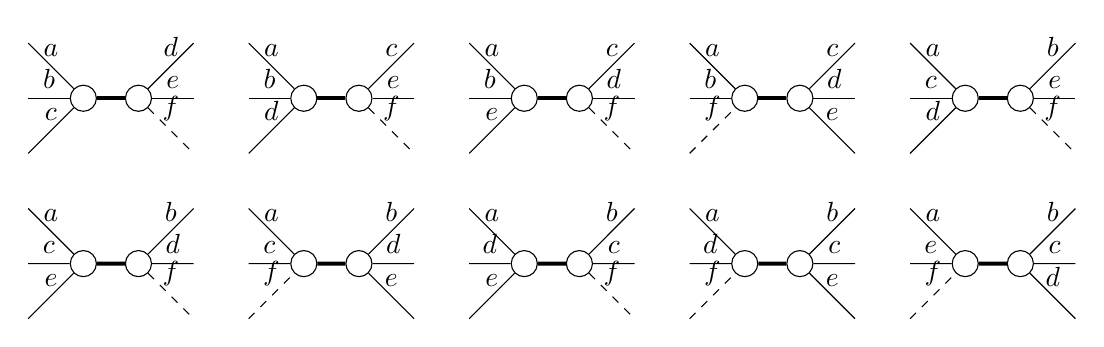
\begin{tikzpicture}[scale=0.7]
\tikzstyle{vertex}=[draw,shape=circle]
\path (0,0) node[vertex](x1){} (1,0) node[vertex](y1){};
\draw[line width=1.5pt] (x1) -- (y1);
\draw[] (-1,1) -- node[above] {$a$} (x1);
\draw[] (-1,0) -- node[above] {$b$} (x1);
\draw[] (-1,-1) -- node[above] {$c$} (x1);
\draw[] (y1) -- node[above] {$d$} (2,1);
\draw[] (y1) -- node[above] {$e$} (2,0);
\draw[dashed] (y1) -- node[above] {$f$} (2,-1);

\path (4,0) node[vertex](x1){} (5,0) node[vertex](y1){};
\draw[line width=1.5pt] (x1) -- (y1);
\draw[] (3,1) -- node[above] {$a$} (x1);
\draw[] (3,0) -- node[above] {$b$} (x1);
\draw[] (3,-1) -- node[above] {$d$} (x1);
\draw[] (y1) -- node[above] {$c$} (6,1);
\draw[] (y1) -- node[above] {$e$} (6,0);
\draw[dashed] (y1) -- node[above] {$f$} (6,-1);

\path (8,0) node[vertex](x1){} (9,0) node[vertex](y1){};
\draw[line width=1.5pt] (x1) -- (y1);
\draw[] (7,1) -- node[above] {$a$} (x1);
\draw[] (7,0) -- node[above] {$b$} (x1);
\draw[] (7,-1) -- node[above] {$e$} (x1);
\draw[] (y1) -- node[above] {$c$} (10,1);
\draw[] (y1) -- node[above] {$d$} (10,0);
\draw[dashed] (y1) -- node[above] {$f$} (10,-1);

\path (12,0) node[vertex](x1){} (13,0) node[vertex](y1){};
\draw[line width=1.5pt] (x1) -- (y1);
\draw[] (11,1) -- node[above] {$a$} (x1);
\draw[] (11,0) -- node[above] {$b$} (x1);
\draw[dashed] (11,-1) -- node[above] {$f$} (x1);
\draw[] (y1) -- node[above] {$c$} (14,1);
\draw[] (y1) -- node[above] {$d$} (14,0);
\draw[] (y1) -- node[above] {$e$} (14,-1);

\path (16,0) node[vertex](x1){} (17,0) node[vertex](y1){};
\draw[line width=1.5pt] (x1) -- (y1);
\draw[] (15,1) -- node[above] {$a$} (x1);
\draw[] (15,0) -- node[above] {$c$} (x1);
\draw[] (15,-1) -- node[above] {$d$} (x1);
\draw[] (y1) -- node[above] {$b$} (18,1);
\draw[] (y1) -- node[above] {$e$} (18,0);
\draw[dashed] (y1) -- node[above] {$f$} (18,-1);

\path (0,-3) node[vertex](x1){} (1,-3) node[vertex](y1){};
\draw[line width=1.5pt] (x1) -- (y1);
\draw[] (-1,-2) -- node[above] {$a$} (x1);
\draw[] (-1,-3) -- node[above] {$c$} (x1);
\draw[] (-1,-4) -- node[above] {$e$} (x1);
\draw[] (y1) -- node[above] {$b$} (2,-2);
\draw[] (y1) -- node[above] {$d$} (2,-3);
\draw[dashed] (y1) -- node[above] {$f$} (2,-4);

\path (4,-3) node[vertex](x1){} (5,-3) node[vertex](y1){};
\draw[line width=1.5pt] (x1) -- (y1);
\draw[] (3,-2) -- node[above] {$a$} (x1);
\draw[] (3,-3) -- node[above] {$c$} (x1);
\draw[dashed] (3,-4) -- node[above] {$f$} (x1);
\draw[] (y1) -- node[above] {$b$} (6,-2);
\draw[] (y1) -- node[above] {$d$} (6,-3);
\draw[] (y1) -- node[above] {$e$} (6,-4);

\path (8,-3) node[vertex](x1){} (9,-3) node[vertex](y1){};
\draw[line width=1.5pt] (x1) -- (y1);
\draw[] (7,-2) -- node[above] {$a$} (x1);
\draw[] (7,-3) -- node[above] {$d$} (x1);
\draw[] (7,-4) -- node[above] {$e$} (x1);
\draw[] (y1) -- node[above] {$b$} (10,-2);
\draw[] (y1) -- node[above] {$c$} (10,-3);
\draw[dashed] (y1) -- node[above] {$f$} (10,-4);

\path (12,-3) node[vertex](x1){} (13,-3) node[vertex](y1){};
\draw[line width=1.5pt] (x1) -- (y1);
\draw[] (11,-2) -- node[above] {$a$} (x1);
\draw[] (11,-3) -- node[above] {$d$} (x1);
\draw[dashed] (11,-4) -- node[above] {$f$} (x1);
\draw[] (y1) -- node[above] {$b$} (14,-2);
\draw[] (y1) -- node[above] {$c$} (14,-3);
\draw[] (y1) -- node[above] {$e$} (14,-4);

\path (16,-3) node[vertex](x1){} (17,-3) node[vertex](y1){};
\draw[line width=1.5pt] (x1) -- (y1);
\draw[] (15,-2) -- node[above] {$a$} (x1);
\draw[] (15,-3) -- node[above] {$e$} (x1);
\draw[dashed] (15,-4) -- node[above] {$f$} (x1);
\draw[] (y1) -- node[above] {$b$} (18,-2);
\draw[] (y1) -- node[above] {$c$} (18,-3);
\draw[] (y1) -- node[above] {$d$} (18,-4);
\end{tikzpicture}
\end{center}
\caption[Breaking a vertex of degree 5 or 6 into two lower-degree vertices]{Breaking a vertex of degree 5 or 6 into two lower-degree vertices. In the degree-5 case, dashed edge $f$ is not present and the vertex is split into one vertex of degree $3$ and another of degree $4$ connected by a forced edge in bold. In the degree-6 case, dashed edge $f$ is present and the vertex is split into two vertices of degree $4$ connected by a forced edge. If edges $a$ and $b$ are included in the original graph's shortest Hamiltonian cycle, then they must not be adjacent to one another in the final graph. This holds in six of the ten ways of splitting the vertex. \label{fig:degree-5}}
\end{figure}

To deal with degree-5 and degree-6 graphs, we reduce them to the degree-4 case. The complexity of the two cases turns out to be the same; however, for clarity we consider each case separately.

\begin{theorem}
\label{thm:deg5}
There is a bounded-error quantum algorithm which solves the TSP for degree-5 graphs in time $O^*(1.680^n\log^2 L\log \log L)$.
\end{theorem}

\begin{proof}
Our algorithm works by splitting each vertex of degree 5 into one vertex of degree $3$ and another of degree $4$ connected by a forced edge. The forced edges can be included in our quantum algorithm by modifying step 1 of the reduction function so that $F'$ contains all the forced edges created by splitting a vertex of degree-$5$ into two vertices connected by a forced edge. Once all degree-$5$ vertices are split this way, we run the degree-$4$ algorithm. It is intuitive to think that this splitting of the vertices could increase the runtime complexity of the degree-$4$ algorithm, due to $n$ being larger. However, the addition of a forced edge incident to every new vertex means that we do not need to create more branches in the backtracking tree in order to include the new vertex in the Hamiltonian cycle. As a result, the time complexity of the degree-$4$ algorithm will remain the same.

There are $10$ unique ways of splitting a vertex of degree $5$ into one vertex of degree $3$ and another of degree $4$ connected by a forced edge. These ten ways of splitting the vertex are shown in Fig.\ \ref{fig:degree-5} for a vertex incident to edges $a,b,c,d,e$. Without loss of generality, let $a$ and $b$ be the two edges which are part of the Hamiltonian cycle. In order for $a$ and $b$ to also be part of the Hamiltonian cycle in the degree-4 graph produced, $a$ and $b$ cannot be adjacent to one another. Looking at Fig.\ \ref{fig:degree-5}, the split is successful in six of the ten ways of splitting the vertex.

If there are $f$ vertices of degree $5$, then there are $10^f$ possible ways of splitting all such vertices, of which $6^f$ will give the correct solution to the TSP. We can apply D\"urr and H\o yer's quantum algorithm for finding the minimum~\cite{durr1996} to find a splitting that leads to a shortest Hamiltonian cycle, or reporting if no cycle exists, after $O((10/6)^{f/2})$ repeated calls to the degree-4 algorithm. To ensure that the failure probability of the whole algorithm is at most $1/3$, we need to reduce the failure probability of the degree-4 algorithm to $O((10/6)^{-f/2})$, which can be achieved by repeating it $O(f)$ times and returning the minimum-length tour found. The overall runtime is thus
%
\begin{align}
&O^*\left(\left(\frac{10}{6}\right)^{\frac{f}{2}}1.301^n\log L \log \log L\right)\\
 = &O^*(1.680^n\log^2 L \log \log L).
\end{align}
\end{proof}
%
It is also possible to split a vertex of degree $5$ into three vertices of degree $3$ connected by two forced edges. There are $15$ ways of performing this splitting, of which $6$ will succeed. Applying the degree-$3$ algorithm to these reduced graphs finds a runtime of
%
\begin{align}
&O^*\left(\left(\frac{15}{6}\right)^{\frac{f}{2}}1.110^n\log L \log \log L\right)\\
 = &O^*(1.754^n\log^2 L \log \log L)
\end{align}
%
\noindent which performs worse than Theorem \ref{thm:deg5}. We next turn to degree-6 graphs, for which the argument is very similar.

\begin{theorem}
There is a quantum algorithm which solves the TSP for degree-$6$ graphs with failure probability $1/3$ in time $O^*(1.680^n\log^2 L \log \log L)$.
\end{theorem}

\begin{proof}
We can extend the idea of Theorem \ref{thm:deg5} to degree-6 graphs by splitting vertices of degree $6$ into two vertices of degree $4$ connected by a forced edge. Because the degree of both new vertices is $4$, there are $\binom{6}{3}/2 = 10$ unique ways of partitioning the edges, of which 4 will fail. We show this in Fig.\ \ref{fig:degree-5} by including the dashed edge $f$ as the sixth edge. The overall runtime is the same as the degree-$5$ case.
\end{proof}

\subsection{Degree-7 graphs}

We next consider extending the algorithm to degree-7 graphs by partitioning degree-7 vertices into one of degree $5$ and another of degree $4$, connected by a forced edge. We can split a vertex of degree $7$ into a vertex of degree $4$ and another of degree $5$ in $\binom{7}{4} = 35$ ways, of which $\binom{7-2}{4-2} + \binom{7-2}{3-2} = 15$ will not preserve the shortest Hamiltonian cycle. We then use the same process as for the degree-5 and degree-6 case, halting after $O((35/20)^{k/2})$ iterations and returning either the shortest Hamiltonian cycle found or reporting if no Hamiltonian cycle exists. From this, our overall runtime is
%
\begin{align}
&O^*\left(\left(\frac{35}{20}\right)^{k/2}1.680^n\log^2 L \log \log L\right)\\
=&O^*(2.222^n\log L \log \log L).
\end{align}
%
This is the point where we no longer see a quantum speedup over the fastest classical algorithms using this approach, as classical algorithms such as those of Held-Karp~\cite{held1962} and Bj{\"o}rklund et al.~\cite{bjorklund2008} run in $O^*(2^n)$ and $O^*(1.984^n)$ time, respectively.

\section{Arbitrary degree graphs}
\label{sec:arbitrary-degree}

We conclude this section with a brief note on what speedups can be obtained from graphs of arbitrary degree. To achieve a speedup, we can apply the quantum speedup for dynamic programming by Ronagh \cite{ronagh2019} to the algorithm of Bj\"orklund et al.\ for graphs of degree $k$ \cite{bjorklund2008}.

The Bj\"orklund et al.\ algorithm runs in the same way as the Held-Karp algorithm, but with an additional polynomial-time circuit that checks if $D(S,l)$ is actually solvable. Adding this same polynomial-time circuit to Ronagh's speedup for the Travelling Salesman Problem will give a speedup of

\begin{equation}
O^*\left(L^4\left(2^{k+1}-2k-2\right)^{n/(2k+2)}\right).
\end{equation}

Runtimes for small instances of $k$ are given in Table \ref{tab:degree-k}, with classical runtimes from Bj"orklund et al.~\cite{bjorklund2008}. It is worth noting that the quantum runtime is strictly less than $O(2^{n/2})$ for all constant $k$. Also note that for $L=\poly(n)$, this runtime is better than the runtimes given in Theorem \ref{thm:deg6}.

\begin{table}
\begin{center}
\begin{tabularx}{\textwidth}{|c|c|C|c|}
\hline Degree $k$ & Quantum & Classical (poly space) & Classical (exp space) \\
\hline 5 & $O^*(1.390^n L^4)$ & $O^*(1.989^n\log L)$ & $O^*(1.932^n\poly(L))$ \\
 6 & $O^*(1.403^n L^4)$ & $O^*(1.996^n\log L)$ & $O^*(1.967^n\poly(L))$\\
 7 & $O^*(1.409^n L^4)$ & $O^*(1.998^n L\log L)$ & $O^*(1.984\poly(L))$ \\
 8 & $O^*(1.411^n L^4)$ & $O^*(1.999^n L\log L)$ & $O^*(1.991\poly(L))$ \\
\hline
\end{tabularx}
\end{center}
\caption[Runtimes of the quantum speedup of Bj\"orklund et al.]{Runtimes of the quantum speedup achieved by applying the quantum speedup of dynamic programming by Ronagh to the bounded-degree TSP algorithm of Bj\"orklund et al. Classical runtimes given in Bj\"orklund et al.\ \cite{bjorklund2008}.}
\label{tab:degree-k}
\end{table}

\section{Conclusion}

In this work we have given examples of where quantum algorithms can provide polynomial (up to quadratic) speedups for the Travelling Salesman Problem in the NP-hard case of bounded-degree graphs. In particular, we are able to offer polynomial speedups for graphs of up to degree 6 in general, and speedups for graphs of arbitrary bounded degree when the edge weights are at most $\poly(n)$. Furthermore, the quantum computing space requirements of all our algorithms are polynomial.

Since the initial publication of the main results in this work a number of other results along these lines have arisen independently \cite{ambainis2018, ronagh2019, ge2019}. We note from Section \ref{ssec:q-dynamic} that the algorithm of Ambainis et al.\ has a runtime of $O^*(1.728^n\log L)$, and therefore does not perform better than our algorithm for degree below 7. Another cost with Ambainis' algorithm is that the algorithm requires an exponentially large amount of space, in order to store all optimal subpaths of length $n(1-\alpha)/4$ in a quantum random access memory. Ronagh's algorithm does perform better then our original algorithm, with a runtime of $O*(2^{n/2}L^4)$, though only for degree-5 and degree-6 graphs, and even then only when the edge weights of the graph are bounded by $\poly(n)$. Furthermore, we argue in Section \ref{sec:arbitrary-degree} that it is possible to adapt Ronagh's original algorithm to the bounded degree setting to provide even better performance. We will discuss the algorithm of Ge and Dunjko more in Section \ref{sec:error-correction}, but for the meantime note that it has a runtime of at best $O^*(2^{n/4})$, which matches the runtime of D\"{o}rn \cite{dorn2007} given in Section \ref{sec:backtrack-tsp} but is slower than our result.

There are several interesting further questions with this research. One is the question of whether or not these algorithms can offer speedups for degree-7 graphs and beyond. On the one hand, in principle any improvements to the classical backtracking algorithms in lower-degree cases will naturally lead to an improvement in the higher-degree cases, due to the reductions. On the other hand, there is a large jump in performance required to move from $O^*(2.222^n\polylog L)$ to $O^*(1.984^n\log L)$, and an even larger one to beat the $O^*(1.728^n\log L)$ runtime of Ambainis et al.~\cite{ambainis2018}. And even if such an improvement is made, there will eventually be a degree at which our current algorithm will not perform better, due to the exponential overhead required for the reduction.

Another interesting question is what other classical algorithms for these problems can be sped up. There are several algorithms which could be interestin in this regard. One example is cut-and-count algorithms which use a combination of Monte-Carlo and dynamic programming \cite{bjorklund14,bodlaender15,cygan11}. Both of these subroutines have quantum speedups \cite{montanaro2015mc, ronagh2019}, but it is unclear if they can both be applied to these algorithms. Another example are branch-and-bound and branch-and-cut algorithms such \cite{little1963, padberg1991}, which offers the best current classical algorithm for solving the Travelling Salesman Problem in practice \cite{applegate2006}. Again, quantum speedups exist for these algorithms \cite{montanaro2019}. However, performance of these algorithms is evaluated by implementing and benchmarking the algorithms, rather than by analytical means. To determine speedups available would require a (logical) gate and qubit decomposition of the quantum algorithm, which is the main challenge.
